\section [Cation Exchange (1D)]{1D reactive transport simulation of cation exchange process}
\label{benchmark_1d_cation_exchange}

\subsection{Definition}
This test example is taken from the PHREEQC User's Guide \cite{Parkhurst1999}.   The simulation is made in order to reproduce the transport of solutes by saturated flow with the influence of cation exchange. The aim of the example is to check the correctness of the coupling between \GeoSys~and PHREEQC by comparing the results of the simulations of both programs. With the calculation model the chemical composition of the effluent from a column containing a cation exchanger and a sodium-potassium-nitrate-solution is simulated. This column is flushed with 3 pore volumes of calcium chloride solution.
~~\\
The 8.2~cm long column contains a sodium-potassium-nitrate solution that is in equilibrium with a cation exchanger. For the one-dimensional calculation the calculation area is simplified as a line. The calculation model includes 82 elements and 83 nodes. As initial condition the water head in the whole domain is given with 2~m. The initial state of the solution is given in table \ref{tab:cationex_chem}.

\begin{table}[htbp]
\centering
\caption{Used parameters}
\begin{tabular}{lll}
\hline
Parameter & Value & Unit \\
\hline
Ca & 0 & $mol \cdot kgw^{-1}$ \\
Cl & 0 & $mol \cdot kgw^{-1}$ \\
K & 2.0$\times 10^{-4}$ & $mol \cdot kgw^{-1}$ \\
Na & 1.0$\times 10^{-3}$ & $mol \cdot kgw^{-1}$ \\
N(5) & 1.2$\times 10^{-3}$ & $mol \cdot kgw^{-1}$ \\
pH & 7 & -- \\
pe & 12.5 & -- \\
Na-X & 5.493$\times 10^{-4}$ & $mol \cdot kgw^{-1}$ \\
K-X & 5.507$\times 10^{-4}$ & $mol \cdot kgw^{-1}$ \\
Ca-X$_2$ & 0 & $mol \cdot kgw^{-1}$ \\
\hline
\end{tabular}
\label{tab:cationex_chem}
\end{table}

{\small
with
\begin{tabbing}
\=xxxxxxx \=xxxxxxxxxxxxxxxxxx \kill
\> pe \> - redox potential \\
\> X \> - ion exchanger \\
\> kgw \> - kilogram of water. \\
\end{tabbing}
}

At the right border of the model the constant head is given with 2~m. At the left border a constant flux of 1.388$\times 10^{-6}$~m$^3\cdot s^{-1}$ is defined as source term. The concentration of this infiltrating CaCl$_2$-solution as well as the pH and pe are given in table \ref{tab:cationex_infil}.

\begin{table}[htbp]
\centering
\caption{State of the infiltration solution}
\begin{tabular}{lll}
\hline\noalign{\smallskip}
\hline
Parameter & Value & Unit \\
\hline
Ca & 6.0$\times 10^{-4}$ & $mol \cdot kgw^{-1}$ \\
Cl & 1.2$\times 10^{-3}$ & $mol \cdot kgw^{-1}$ \\
pH & 7 & -- \\
pe & 12.5 & -- \\
\hline
\end{tabular}
\label{tab:cationex_infil}
\end{table}

The soil material is specified by the parameters in table \ref{tab:cationex_soil}. The dispersion of the transported solutes in this soil is set equal to $2 \cdot 10^{-3}~m$. The calculation is divided in 480 time steps with a constant time step length of 180 seconds. That means, the flow and transport processes in the aquifer within 1 day are simulated.

\begin{table}[htbp]
\centering
\caption{Soil parameters}
\begin{tabular}{lll}
\hline\noalign{\smallskip}
\hline
Parameter & Value & Unit \\
\hline
density $\rho$  & 2000 & $ kg \cdot m^{-3}$  \\
porosity $\Phi$ & 0.5 & -- \\
permeability $K$ & 1.157$\times 10^{-5}$ & $m^2$ \\
\hline
\end{tabular}
\label{tab:cationex_soil}
\end{table}

As this test example has the aim to validate the coupling of \GeoSys~and PHREEQC, merely the comparison between the simulation results of both programs has to be accomplished.

\begin{figure}[htbp]
\centering
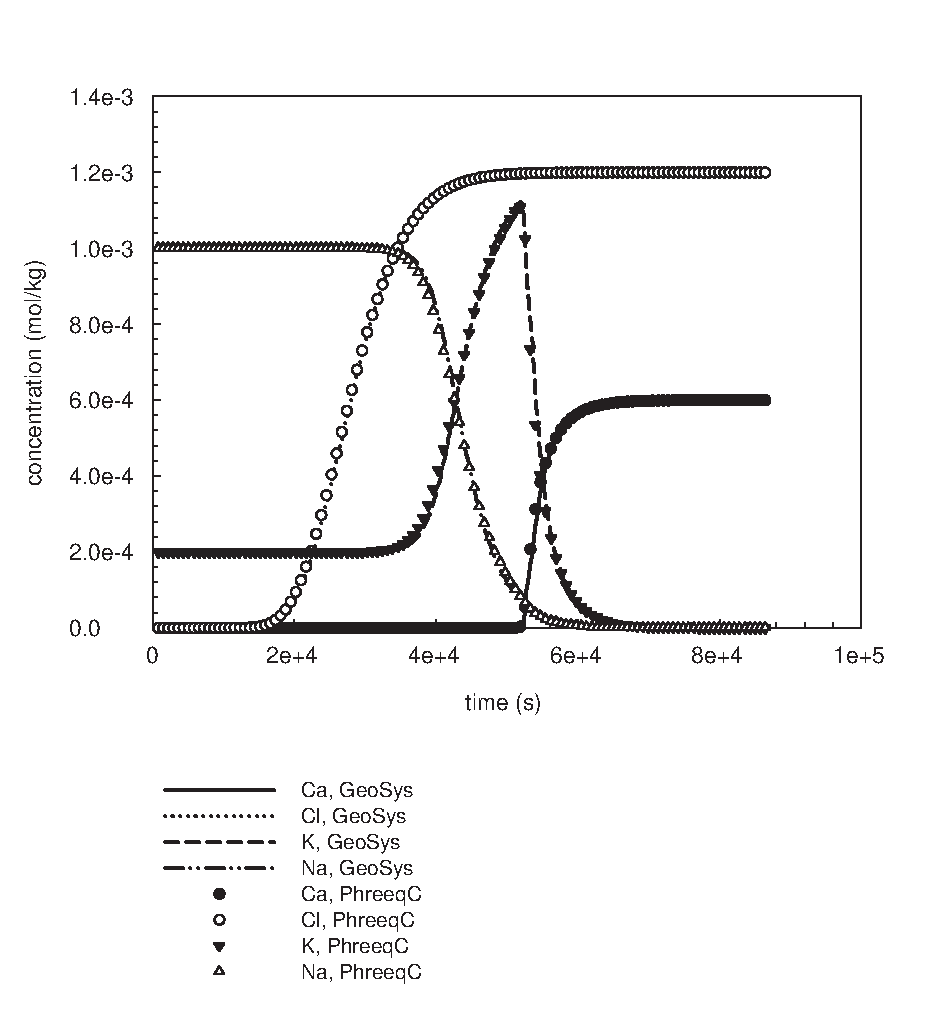
\includegraphics[width=0.8\textwidth]{PART_III/HC/cation_exchange.eps}
\caption{Effluent concentrations  with time of the \GeoSys and PHREEQC simulations}
\label{fig:cationex_output}
\end{figure}

\subsection{Solution}

The numerical results are shown in figure \ref{fig:cationex_output}. The time-dependent concentrations are the values of the compared \GeoSys~and PHREEQC models at the end node and end cell, respectively. Within the calculation time of one day the pore volume of the column model is exchanged three times. As chloride is a conservative tracer it arrives already after the exchange of about one pore volume in the effluent. As long as the exchanger contains sodium this component is eluted. Sodium is initially present in the column and exchanges with the incoming calcium. Potassium is released after sodium. When all of the potassium has been released, the concentration of calcium increases to a steady-state value. As depicted in figure \ref{fig:cationex_output}, between the \GeoSys~and the PHREEQC simulation results there are no differences.

